%%%%%%%%%%%%%%%%%%%%%%%%%%%%% Define Article %%%%%%%%%%%%%%%%%%%%%%%%%%%%%%%%%%
\documentclass{article}
%%%%%%%%%%%%%%%%%%%%%%%%%%%%%%%%%%%%%%%%%%%%%%%%%%%%%%%%%%%%%%%%%%%%%%%%%%%%%%%

%%%%%%%%%%%%%%%%%%%%%%%%%%%%% Using Packages %%%%%%%%%%%%%%%%%%%%%%%%%%%%%%%%%%
\usepackage{geometry}
\usepackage{graphicx}
\usepackage{amssymb}
\usepackage{amsmath}
\usepackage{amsthm}
\usepackage{empheq}
\usepackage{mdframed}
\usepackage{booktabs}
\usepackage{lipsum}
\usepackage{color}
\usepackage{psfrag}
\usepackage{pgfplots}
\usepackage{bm}
%%%%%%%%%%%%%%%%%%%%%%%%%%%%%%%%%%%%%%%%%%%%%%%%%%%%%%%%%%%%%%%%%%%%%%%%%%%%%%%

% Other Settings

%%%%%%%%%%%%%%%%%%%%%%%%%% Page Setting %%%%%%%%%%%%%%%%%%%%%%%%%%%%%%%%%%%%%%%
\geometry{a4paper}

%%%%%%%%%%%%%%%%%%%%%%%%%% Define some useful colors %%%%%%%%%%%%%%%%%%%%%%%%%%
\definecolor{ocre}{RGB}{243,102,25}
\definecolor{mygray}{RGB}{243,243,244}
\definecolor{deepGreen}{RGB}{26,111,0}
\definecolor{shallowGreen}{RGB}{235,255,255}
\definecolor{deepBlue}{RGB}{61,124,222}
\definecolor{shallowBlue}{RGB}{235,249,255}
%%%%%%%%%%%%%%%%%%%%%%%%%%%%%%%%%%%%%%%%%%%%%%%%%%%%%%%%%%%%%%%%%%%%%%%%%%%%%%%

%%%%%%%%%%%%%%%%%%%%%%%%%% Define an orangebox command %%%%%%%%%%%%%%%%%%%%%%%%
\newcommand\orangebox[1]{\fcolorbox{ocre}{mygray}{\hspace{1em}#1\hspace{1em}}}
%%%%%%%%%%%%%%%%%%%%%%%%%%%%%%%%%%%%%%%%%%%%%%%%%%%%%%%%%%%%%%%%%%%%%%%%%%%%%%%

%%%%%%%%%%%%%%%%%%%%%%%%%%%% English Environments %%%%%%%%%%%%%%%%%%%%%%%%%%%%%
\newtheoremstyle{mytheoremstyle}{3pt}{3pt}{\normalfont}{0cm}{\rmfamily\bfseries}{}{1em}{{\color{black}\thmname{#1}~\thmnumber{#2}}\thmnote{\,--\,#3}}
\newtheoremstyle{myproblemstyle}{3pt}{3pt}{\normalfont}{0cm}{\rmfamily\bfseries}{}{1em}{{\color{black}\thmname{#1}~\thmnumber{#2}}\thmnote{\,--\,#3}}
\theoremstyle{mytheoremstyle}
\newmdtheoremenv[linewidth=1pt,backgroundcolor=shallowGreen,linecolor=deepGreen,leftmargin=0pt,innerleftmargin=20pt,innerrightmargin=20pt,]{theorem}{Theorem}[section]
\theoremstyle{mytheoremstyle}
\newmdtheoremenv[linewidth=1pt,backgroundcolor=shallowBlue,linecolor=deepBlue,leftmargin=0pt,innerleftmargin=20pt,innerrightmargin=20pt,]{definition}{Definition}[section]
\theoremstyle{myproblemstyle}
\newmdtheoremenv[linecolor=black,leftmargin=0pt,innerleftmargin=10pt,innerrightmargin=10pt,]{problem}{Problem}[section]
%%%%%%%%%%%%%%%%%%%%%%%%%%%%%%%%%%%%%%%%%%%%%%%%%%%%%%%%%%%%%%%%%%%%%%%%%%%%%%%

%%%%%%%%%%%%%%%%%%%%%%%%%%%%%%% Plotting Settings %%%%%%%%%%%%%%%%%%%%%%%%%%%%%
\usepgfplotslibrary{colorbrewer}
\pgfplotsset{width=8cm,compat=1.9}
%%%%%%%%%%%%%%%%%%%%%%%%%%%%%%%%%%%%%%%%%%%%%%%%%%%%%%%%%%%%%%%%%%%%%%%%%%%%%%%

%%%%%%%%%%%%%%%%%%%%%%%%%%%%%%% Title & Author %%%%%%%%%%%%%%%%%%%%%%%%%%%%%%%%
\title{Virtual Lab for Numerical Aperture of an Optical Fiber}
\author{Ashraf Syed, Rammohan M, Tejas Kotte Reddy, Pranaov S}
%%%%%%%%%%%%%%%%%%%%%%%%%%%%%%%%%%%%%%%%%%%%%%%%%%%%%%%%%%%%%%%%%%%%%%%%%%%%%%%



\begin{document}
\maketitle
\tableofcontents
\newpage


\section{Introduction to Optical Fiber}


Optical fiber is a type of flexible, transparent fiber made of transparent dielectric (glass or plastic) that is used to transmit light signals over long distances. It works based on the principle of total internal reflection, where light is bounced inside the fiber, allowing it to travel through even long, curved paths without significant loss of signal. It is as thin as human hair, approximately 70 micrometers (0.003 inch) in diameter.


\begin{figure}[h]
    \centering
    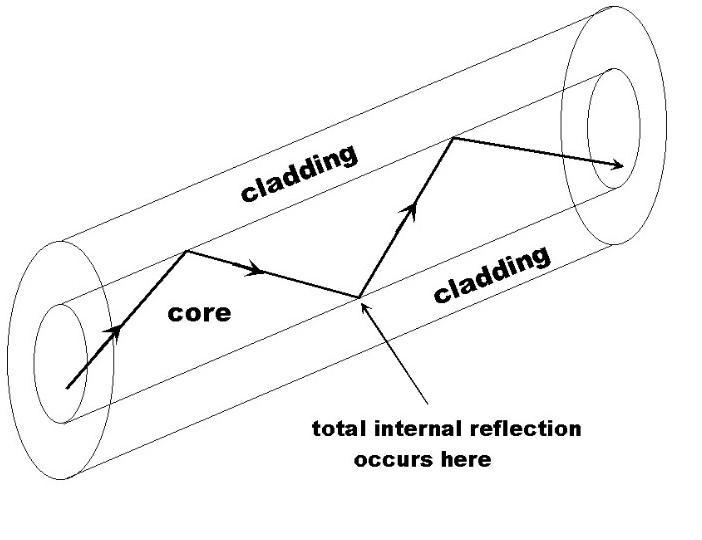
\includegraphics[width=0.8\textwidth]{./assets/optical-fiber.jpg}
    \caption{Optical Fiber}
    \label{fig:optical-fiber}
\end{figure}

\subsection{Refractive index}


The refractive index, also known as the index of refraction, is a measure of how much a material slows down and bends light as it passes through that material. It indicates the speed at which light travels in a medium compared to its speed in a vacuum.

\subsubsection{Formula}

The refractive index is defined as the ratio of the speed of light in a vacuum to the speed of light in the material:
\[
n = \frac{c}{v}
\]
where:
\begin{itemize}
    \item \( n \) is the refractive index of the material
    \item \( v \) is the speed of light in the material
    \item \( c \) is the speed of light in a vacuum
\end{itemize}



\subsection{Core and Cladding}

The core and cladding are the two primary components of optical fiber that work together to transmit light signals efficiently.

\subsubsection{Core}

\textbf{Function:} The core is the central part of the optical fiber through which light travels. It carries the actual data in the form of light signals.

\textbf{Material:} The core is typically made of glass or plastic with a high refractive index. The refractive index is the measure of how much light bends when entering the material. A higher refractive index in the core ensures that light can be trapped and guided along the fiber.

\textbf{Size:} The core's diameter varies depending on the type of optical fiber:
\begin{itemize}
    \item In single-mode fiber (SMF), the core is typically around 8-10 micrometers in diameter.
    \item In multi-mode fiber (MMF), the core is much larger, typically between 50-100 micrometers in diameter.
\end{itemize}

\subsubsection{Cladding}

\textbf{Function:} The cladding surrounds the core and helps keep the light inside the core by creating a boundary that causes the light to reflect back into the core. This is done through a process called total internal reflection, which ensures that light remains confined to the core as it travels along the fiber.

\textbf{Material:} The cladding is usually made from glass or plastic, but with a lower refractive index than the core. This difference in refractive indices between the core and cladding is what causes the light to reflect internally and not escape.

\textbf{Structure:} The cladding is typically several micrometers thick and serves as a protective layer for the core, preventing physical damage and contamination.

\subsubsection{How They Work Together}

When light travels through the core, it hits the boundary between the core and cladding at a steep angle. Because the core has a higher refractive index than the cladding, the light bounces off the boundary and remains within the core. This ensures that the light signal continues to travel through the fiber without escaping into the surrounding environment.

\textbf{Signal Guidance:} By confining the light within the core and using total internal reflection, the fiber can transmit data over long distances with minimal signal loss or degradation.

\section{Total Internal Reflection}

A medium having a lower refractive index is said to be an optically rarer medium while a medium having a higher refractive index is known as an optically denser medium. When a ray of light passes from a denser medium to a rarer medium, it is bent away from the normal in the rarer medium (see Fig. \ref{fig:total-internal-reflection}). Snell's law for this case may be written as:
\[
\sin \theta_2 = \left(\frac{n_1}{n_2}\right) \sin \theta_1
\]
where \(\theta_1\) is the angle of incidence of the light ray in the denser medium and \(\theta_2\) is the angle of refraction in the rarer medium. Also, \(n_1\) and \(n_2\) are the refractive indices of the denser and rarer media, respectively.

When the angle of incidence, \(\theta_1\), in the denser medium is increased, the transmission angle, \(\theta_2\), increases and the refracted rays bend more and more away from the normal. At some particular angle \(\theta_C\), the refracted ray glides along the boundary surface so that \(\theta_2 = 90^\circ\), as seen in Fig. \ref{fig:critical-angle}. At angles greater than \(\theta_C\), there are no refracted rays at all. The rays are reflected back into the denser medium as though they encountered a specular reflecting surface (Fig. \ref{fig:total-internal-reflection}). Thus,

\begin{itemize}
    \item If \(\theta_1 < \theta_C\), the ray refracts into the rarer medium.
    \item If \(\theta_1 = \theta_C\), the ray just grazes the interface of the rarer-to-denser media.
    \item If \(\theta_1 > \theta_C\), the ray is reflected back into the denser medium.
\end{itemize}

The phenomenon in which light is totally reflected from a denser-to-rarer medium boundary is known as total internal reflection. The rays that experience total internal reflection obey the laws of reflection. Therefore, the critical angle can be determined from Snell's law.

\begin{figure}[ht]
    \centering
    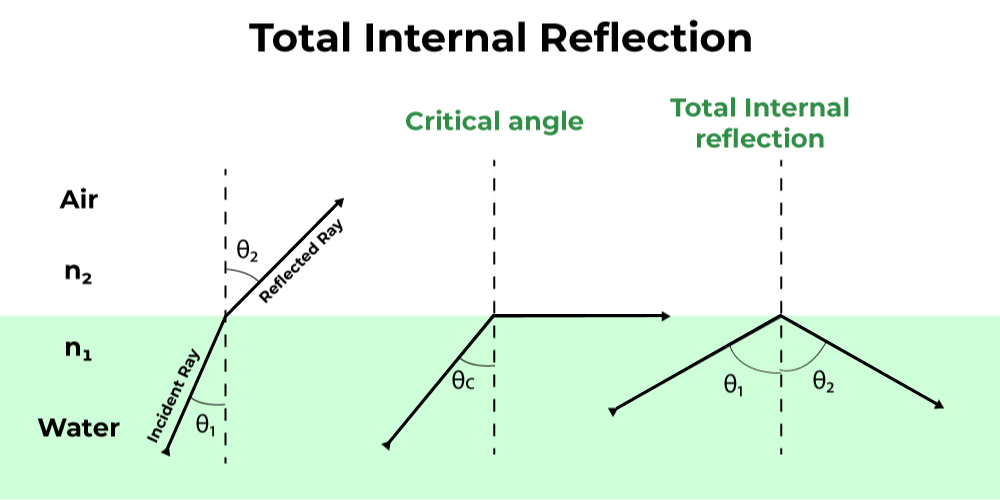
\includegraphics[width=0.8\textwidth]{assets/total-internal-reflection.jpg}
    \caption{Total Internal Reflection}
    \label{fig:total-internal-reflection}
\end{figure}

\begin{figure}[ht]
    \centering
    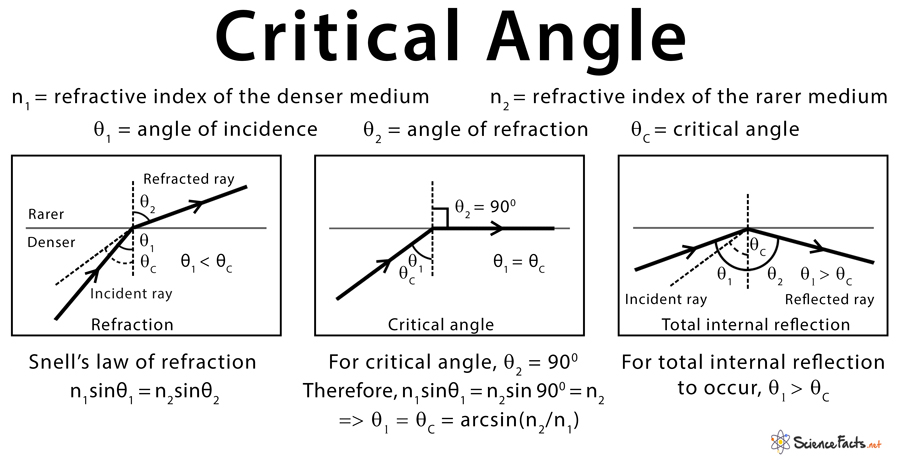
\includegraphics[width=0.8\textwidth]{assets/critical-angle.jpg}
    \caption{Critical Angle}
    \label{fig:critical-angle}
\end{figure}

\subsection{Acceptance angle}

Let us again consider a step index optical fibre into which light is launched at one end. Let the refractive index of the core be \(n_{1}\) and the refractive index of the cladding be \(n_{2}\) (\(n_{2} < n_{1}\)).

Let \(n_{0}\) be the refractive index of the medium from which light is launched into the fibre. Assume that a light ray enters the fibre at an angle \(\theta_{0}\) to the axis of the fibre. The ray refracts at an angle \(\theta_{1}\) and strikes the core-cladding interface at an angle \(\theta_{2}\). If \(\theta_{2}\) is greater than the critical angle, the ray undergoes total internal reflection at the interface, since \(n_{1} > n_{2}\). As long as the angle \(\theta_{2}\) is greater than the critical angle, the light will stay within the fibre.

Applying Snell's law to the launching face of the fibre, we get
\[
n_{0} \sin \theta_{0} = n_{1} \sin \theta_{1}
\]

If \(\theta_{0}\) is increased beyond a limit, \(\theta_{2}\) will drop below the critical value and the ray escapes from the sidewalls of the fibre. The largest value of \(\theta_{0}\) occurs when \(\theta_{2} = \theta_{c}\). From the triangle ABC, it is seen that
\[
\sin \theta_{c} = \frac{n_{2}}{n_{1}}
\]

The angle \(\theta_{0}\) is called the acceptance angle of the fibre.

Acceptance angle is the maximum angle that a light ray can have relative to the axis of the fibre and propagate down the fibre.

Thus, only those rays that are incident on the face of the fibre making angles less than \(\theta_{0}\) will undergo repeated total internal reflections and reach the other end of the fibre. Obviously, larger acceptance angles make it easier to launch light into the fibre.

In three dimensions, the light rays contained within the cone having a full angle \(2\theta_{0}\) are accepted and transmitted along the fibre. Therefore, the cone is called the acceptance cone.

Light incident at an angle beyond \(\theta_{0}\) refracts through the cladding and the corresponding optical energy is lost.


\subsection{Critical Angle}

The critical angle is a key concept in the study of optical fibers and total internal reflection. It is defined as the angle of incidence in the denser medium at which the angle of refraction in the rarer medium is \(90^\circ\). Beyond this angle, light is completely reflected back into the denser medium, a phenomenon known as total internal reflection.

\section{Measurement of Numerical Aperture}


\subsection{Apparatus}

The following apparatus are required for the experiment:
\begin{itemize}
    \item Laser source or LED
    \item Numerical aperture apparatus
    \item Numerical aperture jig
    \item Cable
    \item Screen
    \item Fiber optic cable
\end{itemize}

\subsection{Description of the Experiment}

An LED or laser source is coupled to the input of the optical fiber. The numerical aperture jig holds the output of the fiber, where light falls onto a movable screen consisting of circular rings of varying diameters in millimeters. A scale is fixed at the bottom to measure the distance from the screen to the laser output. The screen is moved to different lengths \(L\), and the corresponding diameter \(W\) is noted. The formula for numerical aperture (NA) is given by:

\[
\text{NA} = \sin \theta = \frac{W}{\sqrt{4L^2 + W^2}}
\]
\[
  \text{Accpetance angle } \theta = \sin^{-1}\frac{W}{\sqrt{4L^2 + W^2}}
\]

\subsection{Procedure}

\begin{enumerate}
    \item Couple the LED or laser source to the input of the optical fiber.
    \item Secure the numerical aperture jig at the output of the fiber.
    \item Position the movable screen with circular rings at a known distance \(L\) from the fiber output.
    \item Measure the diameter \(W\) of the light spot on the screen.
    \item Repeat the measurements for different lengths \(L\).
    \item Calculate the numerical aperture using the formula provided.
\end{enumerate}

\subsection{Results and Analysis}

Record the measurements of \(L\) and \(W\) in a table and calculate the numerical aperture for each set of measurements. Analyze the results to determine the accuracy and efficiency of the optical fiber in guiding light signals.

\end{document}
